% This file is for chapter 2

\chapter{Theoretical Background}

\section{My First Section}

This first work theoretical in this area was performed by Golomb
\cite{Golomb82}. This is meaningless text used only to test the
margins and such. This is meaningless text used only to test the
margins and such. This is meaningless text used only to test the
margins and such.
\subsection{A Subsection}
Bringing this work to practical fruition has been attributed to
Dixon \cite{Dixon94}. This is meaningless text used only to test
the margins and such. This is meaningless text used only to test
the margins and such. This is meaningless text used only to test
the margins and such. 
\subsection{Another Subsection}
Let's try out an equation. The expression for a double-sideband
(with carrier) AM signal is
\begin{equation}
s_{\mathrm{AM}}(t)=A_c[1+m(t)]\cos(\omega_c t) \label{eq:dsb_lc}
\end{equation}
where $A_c$ is the amplitude of the carrier, $m(t)$ is the message
signal (with amplitude always $\le 1$ to prevent overmodulation),
and $\omega_c$ is the carrier frequency expressed in radians/sec
\cite{Couch01}. In order to recover the message signal from
(\ref{eq:dsb_lc}), it is necessary to extract the envelope of the
signal $A_c[1+m(t)]$. Once the envelope is obtained, the DC
component can be removed with a DC blocking filter, leaving $A_c
m(t)$, which is a scaled version of the original message signal.
This is meaningless text used only to test the margins and such.
This is meaningless text used only to test the margins and such.
This is meaningless text used only to test the margins and such.
This is meaningless text used only to test the margins and such.
This is meaningless text used only to test the margins and such.

\section{My Second Section}

Let's see how a floating figure is formatted.  As we see in
Figure~\ref{fg:ctf}, the optical measures of MTF and CTF are
not equal \cite{smith90}.
\begin{figure}
\centering
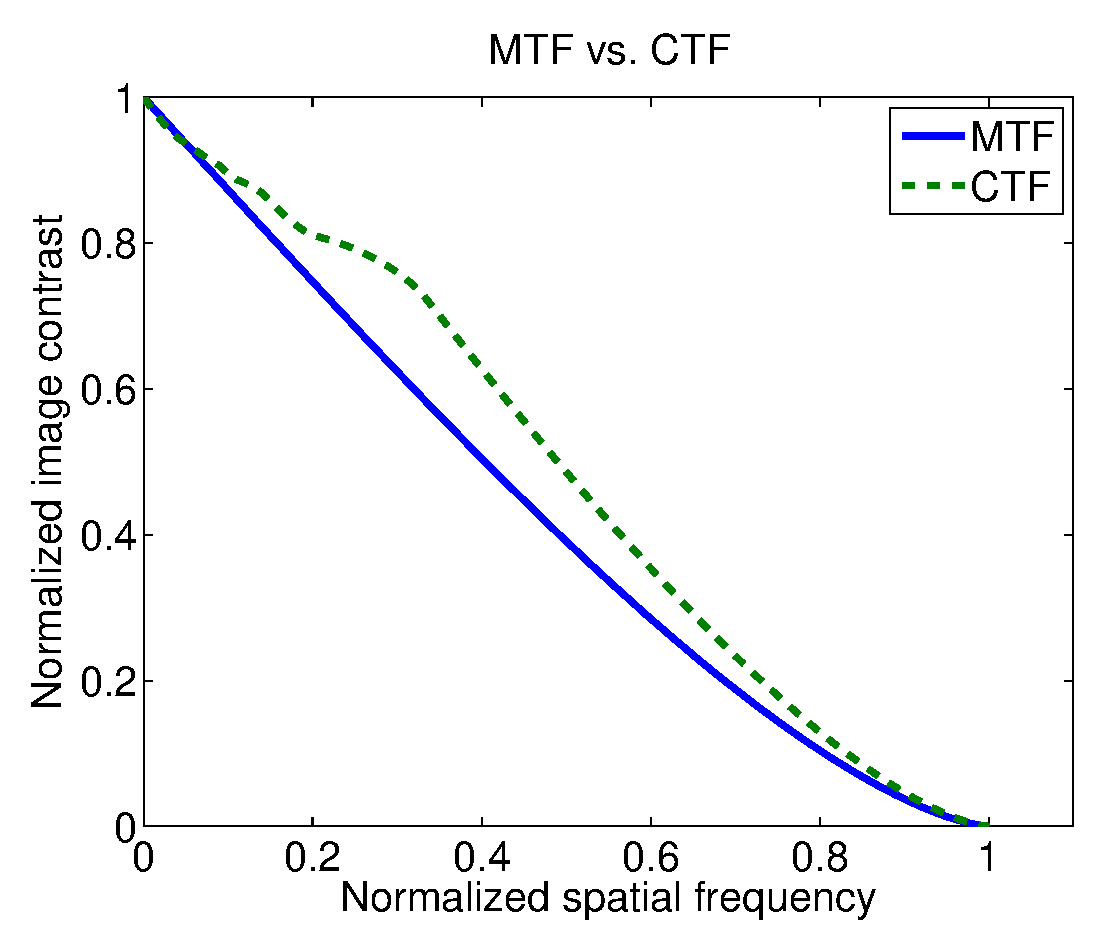
\includegraphics[width=0.7\textwidth]{ctf.eps}
\caption[MTF versus CTF.]{A comparison of the modulation transfer
function and the contrast transfer function.} \label{fg:ctf}%
\end{figure}
Note that for a figure environment, the caption comes \emph{after} the
definition of the figure itself.

Sometimes you want to combine two subfigures into one main figure.  The \pc{subfig} package, loaded automatically with the UW thesis and dissertation files, can easily do this.  You just use the \pc{\subfloat} command as shown in the \TeX\ source file below (it won't show up in the PDF file, of course, only the result of the command shows up there).

Some common shapes for individual positive and negative lenses, and their associated names, are shown in Fig.~\ref{fg:lens_types}.  
\begin{figure}%
\centering
\subfloat[Positive (converging) lenses.]{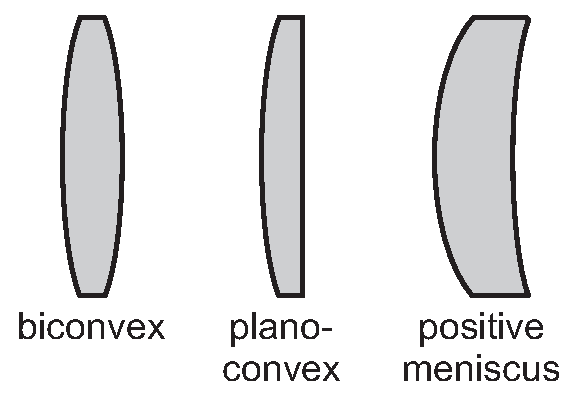
\includegraphics[width=0.35\textwidth]{lens_positive3.eps}}\qquad\qquad
\subfloat[Negative (diverging) lenses.]{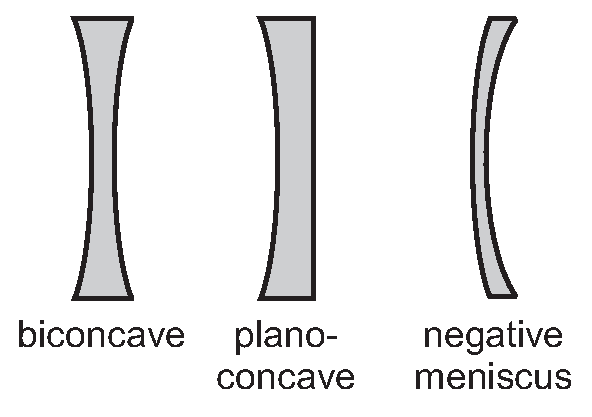
\includegraphics[width=0.35\textwidth]{lens_negative3.eps}}
\caption{Common types of lenses.}
\label{fg:lens_types}
\end{figure}

How about listings of computer programs? The main program
(\pc{main.c}) is very basic, as shown below. Note that unless your
advisor objects, program listings should be single-spaced, which
can be controlled with the \pc{\spacing} command as shown.  If you 
have longer and/or many program listings, it's usually better to 
place them in an appendix.

\begin{spacing}{1}
\begin{lstlisting}[caption={Main program for simple frame-based processing
  using ISRs.},label={cd:FrameMain_isr}]{}
#include "..\Common_Code\DSK_Config.h" 
#include "frames.h"

int main() {
    // initialize all buffers to 0
    ZeroBuffers();

    // initialize DSK for selected codec
    DSK_Init(CodecType, TimerDivider);

    // main loop here, process buffer when ready
    while(1) {
        if(IsBufferReady()) // process buffers in background
            ProcessBuffer();
    }
}
\end{lstlisting}
\end{spacing}
\noindent Wasn't that a nice program?  % see how to avoid an indented line?

How about some \ml\ code? Note you have to specify the language
since \ml\ wasn't the default language in the ``listings'' setup.

\begin{spacing}{1}
\begin{lstlisting}[language=matlab,%
caption={Simple \ml\ FIR filter example.}]{}
%  This m-file is used to convolve x[n] and B[n]
%
%  Assumes that both x[n] and B[n] start at n = 0
%
%  written by Dr. Thad B. Welch, PE {t.b.welch@ieee.org}
%  copyright 2001
%  completed on 13 December 2001 revision 1.0

% Simulation inputs
x = [1 2 3 0 1 -3 4 1];             % input vector x[n]
B = [0.25 0.25 0.25 0.25];          % FIR filter coefficients B[n]

% Calculated terms
PaddedX = [x zeros(1,length(B)-1)]; % zeros pads x[n] to flush the filter
n = 0:(length(x) + length(B) - 2);  % plotting index for the output
y = filter(B, 1, PaddedX);          % performs the convolution

% Simulation outputs
stem(n, y)                          % output plot generation
ylabel(`output values')
xlabel(`sample number')
\end{lstlisting}
\end{spacing}

New paragraph. This is meaningless text used only to test the
margins and such. This is meaningless text used only to test the
margins and such. This is meaningless text used only to test the
margins and such. This is meaningless text used only to test the
margins and such. This is meaningless text used only to test the
margins and such. This is meaningless text used only to test the
margins and such. This is meaningless text used only to test the
margins and such. This is meaningless text used only to test the
margins and such. This is meaningless text used only to test the
margins and such. This is meaningless text used only to test the
margins and such. This is meaningless text used only to test the
margins and such. This is meaningless text used only to test the
margins and such. This is meaningless text used only to test the
margins and such.

\section{My Third Section}

Now let's see how a table is formatted. The minimum distance to a
nearest cluster point is given in Table~\ref{tb:results3}.
% uncomment the [!b] below if you *really want the table placed at the bottom of the page
\begin{table}%[!b]
\begin{center}
\caption[Results of the experiment testing for recognition of
occluded objects.]{Results of the third experiment, showing
Euclidean distance to nearest eigenspace model point. Smaller
numbers represent ``better'' recognition. This experiment tested
for recognition of occluded objects.\\}
 \label{tb:results3}
\begin{tabular}{c|c c c} \hline
  & Occluded F4 & Occluded F14 & Occluded Tornado \\ \hline
  Tornado & 13.8922 & 6.4154 & {\bf 68.9262}\\
  P51 & 6.7955 & 3.7622 & 53.9320 \\
  F4 & {\bf 5.7648} & 5.5956 & 48.3343 \\
  F14 & 6.9371 & {\bf 3.9662} & 48.2957 \\
  F22 & 4.8605 & 5.6179 & 45.3576 \\ \hline
\end{tabular}
\end{center}
\end{table}
Note that for a table environment, the caption comes \emph{before} the
definition of the table itself.

This is meaningless text used only to test the margins and such.
This is meaningless text used only to test the margins and such.
This is meaningless text used only to test the margins and such.
This is meaningless text used only to test the margins and such.
This is meaningless text used only to test the margins and such.
This is meaningless text used only to test the margins and such.
This is meaningless text used only to test the margins and such.
This is meaningless text used only to test the margins and such.


% Cheat to bring in other references
\nocite{*} % delete or comment this out.
